\documentclass{article}


\usepackage{PRIMEarxiv}

\usepackage[utf8]{inputenc} % allow utf-8 input
\usepackage[T1]{fontenc}    % use 8-bit T1 fonts
\usepackage{hyperref}       % hyperlinks
\usepackage{url}            % simple URL typesetting
\usepackage{booktabs}       % professional-quality tables
\usepackage{amsfonts}       % blackboard math symbols
\usepackage{nicefrac}       % compact symbols for 1/2, etc.
\usepackage{microtype}      % microtypography
\usepackage{lipsum}
\usepackage{fancyhdr}       % header
\usepackage{graphicx}       % graphics
\graphicspath{{media/}}     % organize your images and other figures under media/ folder

% Add these additional useful packages
\usepackage{amsmath}    % For better math formatting
\usepackage{amsthm}     % For theorem environments
\usepackage{geometry}   % Already included but should be with other formatting packages
\usepackage{cleveref}   % For better reference handling

% Better header setup
\pagestyle{fancy}
\fancyhf{} % clear all header and footer fields
\fancyhead[L]{Q-Learning Implementation for Flappy Bird}
\fancyhead[R]{\thepage}
\renewcommand{\headrulewidth}{0.4pt}

% Better math spacing in equations
\setlength{\abovedisplayskip}{10pt}
\setlength{\belowdisplayskip}{10pt}

% Better figure settings
\usepackage{float}
\graphicspath{{images/}{figures/}{media/}} % multiple possible paths for images

% Better itemize spacing
\usepackage{enumitem}
\setlist{nosep} % Reduces vertical spacing in lists

\title{Q-Learning Implementation for Flappy Bird
\thanks{\textit{\underline{Citation}}: 
\textbf{Gulabrao, A. Q-Learning Implementation for Flappy Bird. 2024.}} 
}

\author{
  Akshay Gulabrao \\
  Department of Computer Science \\
  University \\
  City \\
  \texttt{email@university.edu}
}

\date{November 2nd, 2024}

\begin{document}

\maketitle

\begin{abstract}
This paper presents an educational implementation of Q-Learning applied to the mobile game Flappy Bird. Using the Gymnasium framework and a custom environment, we demonstrate how reinforcement learning can be used to teach an agent to play Flappy Bird autonomously. The implementation serves as a practical example of Markov Decision Processes and Q-Learning concepts, making it valuable for students learning about reinforcement learning algorithms.
\end{abstract}

\keywords{Reinforcement Learning \and Q-Learning \and Flappy Bird \and Educational Implementation}

\section{Introduction}
One of the long-standing challenges of computers is the ability to learn from experience. Reinforcement learning (RL) is a field of artificial intelligence that aims to teach computers how to learn by placing them in interactive environments. The computer program (agent) observes the state of an environment and then chooses an action. As a result, the state changes, and the environment informs the agent whether the behavior was optimal through a numerical reward signal. The agent interacts with the environment numerous times to correlate states, actions, and rewards with each other. Ultimately, the agent finds an optimal policy to maximize the cumulative reward over time.

Flappy Bird is a mobile game from 2013 where the user controls a bird to dodge a stream of static obstacles. The bird naturally falls, so the user must balance flight dynamics with obstacle avoidance to periodically "flap" its wings, providing the bird with a burst of acceleration.

The agent can learn how to recognize the state of the bird and determine optimal flapping times using an RL algorithm known as Q-Learning.\cite{Q-Learning} Introduced by Watkins in 1989, Q-Learning enables the agent to leverage previous experiences to choose the best action.

In this educational paper, I implement Q-Learning for Flappy Bird using the open-source library Gymnasium and the environment created by Luptakova et al.\cite{Luptakova}


MDPs provide a formal framework to describe agent interaction.
This interaction is defined with four components: state, actions, rewards, and transition probabilities. 
The state space $S$ is the set of all possible situations that an agent can observe. 
The action space $A$ is the set of all possible actions that an agent can do. 
The reward function $R$ is a function $R(S,A) \rightarrow \mathbb{R}$ which maps a state $S$ and an action $A$ to a scalar reward $R$. 
The transition probability $P(S'|S,A)$ is a function of state $S$ and action $A$ that returns the probability of the next state $S'$.
Figure \ref{fig:chart} provides a representation of how the agent interacts with its environment.

\begin{figure}[H]
\centering
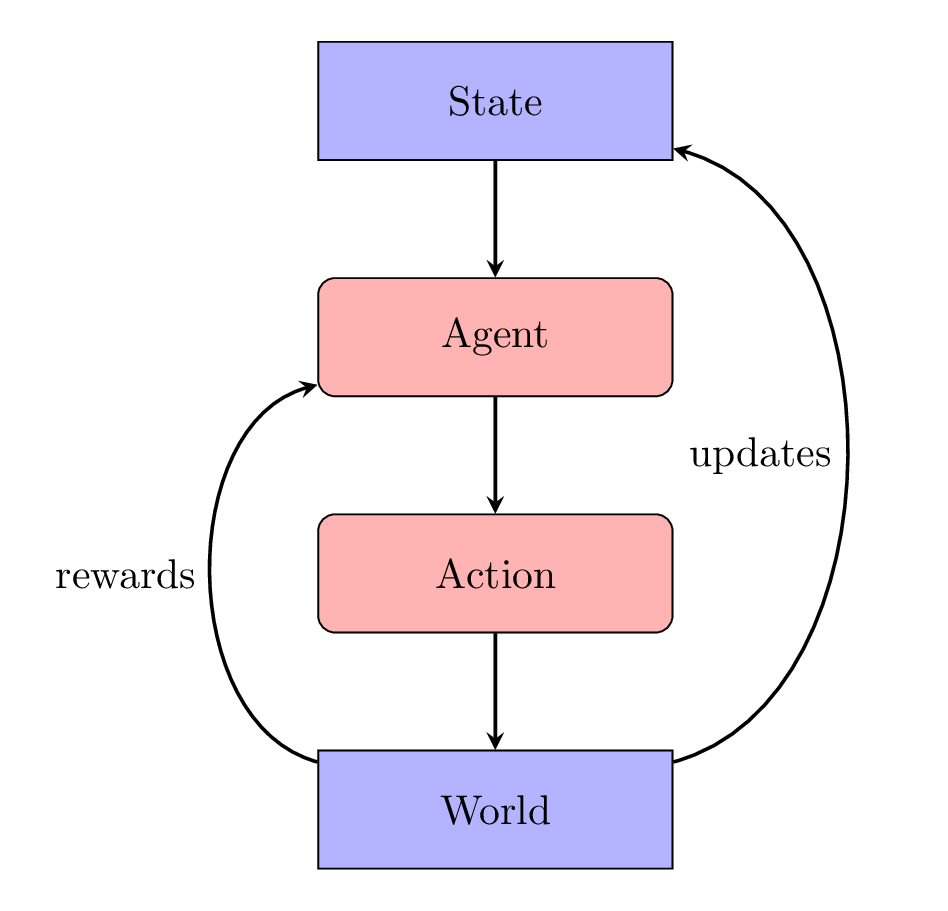
\includegraphics[width=0.7\textwidth]{images/chart.png}
\caption{The agent observes the current state of the world and chooses an action. 
         The world then updates the state and returns a reward to the agent 
         indicating whether the action was desirable.}
\label{fig:chart}
\end{figure}

To demonstrate MDPs in practice, I create an autonomous learning agent which solves the MDP for the Flappy Bird game. Flappy Bird is a good testbench for Reinforcement Learning algorithms because of its finite action space and small state space.

\section{Background}


\subsection{Markov Decision Processes}
An agent's interaction with the environment can be represented as an MDP trajectory. The agent is initially provided the state $S_0$ and must choose an action $A_0$, from which the world will update $S_1$ and $R_1$ for the agent to learn from. The MDP trajectory is a sequence $M$ where

$$M = S_0,A_0,R_1,S_1,A_1,R_2,S_2,A_2, \ldots$$

where:
\begin{itemize}[leftmargin=*]  % Aligns items with text
    \item $t \in \mathbb{N}$ is the timestep
    \item $d$ is the dimension of the world state
    \item $S_t \in \mathbb{R}^d$ is the state at time $t$
    \item $A_t \in \mathbb{N}$ is the action at time $t$
    \item $R_t \in \mathbb{R}$ is the reward at time $t$ for state $(S_{t-1},A_{t-1})$
\end{itemize}

In my implementation of Flappy Bird, the state space is $S \in \mathbb{R}^d$, where $d$ represents coordinates of the last pipe, the next 2 pipes, the player's position, velocity, and rotation.

Every MDP must satisfy the Markov Property, the next state is only dependent on the state prior to it, not any other states. This means that it is possible to compute the optimal action at any given time using only a single state. If the Markov property was not satisfied, then the transition probabilities would need to be computed with $P(S' | S_t,A_t,S_{t-1}, A_{t-1},...)$ instead of $P(S' | S_t,A_t)$. This would make learning the optimal policy orders of magnitude more expensive.

The goal of each learning algorithm is to solve the MDP by finding an optimal policy. A policy is a decision-making function $\pi$ that maps each state to an action. The optimal policy maximizes the expected reward of all future states. A discount rate $\gamma$ is applied to all future states because future states are less certain than immediate states. The expected reward $G$ at time $t$ is then:

$$G_t \doteq R_t + \sum^\infty_{k=1} \gamma^{k}R_{t+k} = \sum^\infty_{k=0}\gamma^kR_{t+k}$$

The agent can model its expected return by using the quality function $q_\pi(s,a)$, which measures the quality of an action $A_t$ in state $S_t$. The expected reward of each action is then

$$q_\pi(s,a) \doteq \mathbb{E}_\pi[G_t|S_t = s,A_t = a] = \mathbb{E}_\pi[\sum^\infty_{k=0}\gamma^kR_{t+k} | S_t = s,A_t = a]$$

\subsection{Bellman Equation}
The Bellman Equation approximates the true value of each state and action, which is the sum of the reward and all future rewards in the current state. The state-action value function $q_\pi$ is computed recursively using the Bellman equation to learn the true state-action function $q^*(s,a)$.

\begin{align}
q_\pi(s,a) &= \mathbb{E}_\pi[G_t|S_t = s,A_t = a] \label{eq:qlearning1} \\
&= \mathbb{E}_\pi[R_t + \gamma G_{t+1} | S_t = s, A_t = a] \notag \\
&= \sum_{s'}\sum_{r}p(s',r|s,a)[r + \gamma\mathbb{E}_\pi[G_{t+1}|S_{t+1} = s', A_{t+1} = a']] \notag \\
&= \sum_{s',r}p(s',r|s,a)[r + \gamma q_\pi(s',a')] \notag
\end{align}

The Bellman Equation requires knowledge of environment dynamics $P(S',R | S,A)$ and the discounted expected return $G_t$, neither of which is available to the agent. Instead the agent must be able to estimate the values through interacting with the environment.

\subsection{Q-Learning}
In Q-Learning, instead of learning an optimal policy, the agent learns the quality function, and then takes the best action in each state. The agent updates $q_\pi(s,a)$ in real time based on the reward received $R_{t+1}$, the new state $S_{t+1}$, and the value of the state $S_{t+1}$,  assuming that the optimal action is taken $\max_aQ_\pi(S_{t+1}, a)$. Q-learning is an off-policy learning algorithm, meaning it can learn the value of the optimal policy regardless of the agent's thinking behind actions since the next state is only dependent on the previous state and the action. If the agent takes action $A_t$ in state $S_t$ then

\begin{equation} \label{eq:qupdate}
\begin{split}
Q_\pi(S_t,A_t) \leftarrow Q_\pi(S_t,A_t) + \alpha&[R_{t+1} + \\
&\gamma\max_aQ_\pi(S_{t+1},a) - Q_\pi(S_t,A_t)]
\end{split}
\end{equation}

where
\begin{itemize}
    \item $\alpha$ is the step-size used to update each state
    \item $\gamma$ is the discount rate of future states
\end{itemize}

\bibliographystyle{plain} % Choose a bibliography style
\bibliography{references} % The name of your .bib file without the extension
\end{document}